\PassOptionsToPackage{lowtilde}{url}
\documentclass[aspectratio=43,english]{beamer} %If you want to create Polish presentation, replace 'english' with 'polish' and uncomment 3-th line, i.e., '\usepackage{polski}'
\usepackage[utf8]{inputenc}
\usepackage{polski} %Uncomment for Polish language
\usepackage{babel}
\usepackage{listings} %We want to put listings

\mode<beamer>{ 	%in 'beamer' mode
	\hypersetup{pdfpagemode=FullScreen}		%Enable Full screen mode
	\usetheme{JuanLesPins} 		%Show part title in right footer
	%\usetheme[dark]{AGH}                 		%Use dark background
	%\usetheme[dark,parttitle=leftfooter]{AGH}  	%Use dark background and show part title in left footer
}
\mode<handout>{	%in 'handout' mode
	\hypersetup{pdfpagemode=None}
	\usepackage{pgfpages}
  	\pgfpagesuselayout{4 on 1}[a4paper,border shrink=5mm,landscape]	%show 4 slides on 1 page
  	\usetheme{boxes}
  	\addheadbox{structure}{\quad\insertpart\hfill\insertsection\hfill\insertsubsection\qquad} 	%content of header
 	\addfootbox{structure}{\quad\insertauthor\hfill\insertframenumber\hfill\insertsubtitle\qquad} 	%content of footer
}

\AtBeginPart{ %At begin part: display its name
	\frame{\partpage}
}


%%%%%%%%%%% Configuration of the listings package %%%%%%%%%%%%%%%%%%%%%%%%%%
% Source: https://en.wikibooks.org/wiki/LaTeX/Source_Code_Listings#Using_the_listings_package
%%%%%%%%%%%%%%%%%%%%%%%%%%%%%%%%%%%%%%%%%%%%%%%%%%%%%%%%%%%%%%%%%%%%%%%%%%%%
\lstset{ %
  backgroundcolor=\color{white},   % choose the background color
  basicstyle=\footnotesize,        % the size of the fonts that are used for the code
  breakatwhitespace=false,         % sets if automatic breaks should only happen at whitespace
  breaklines=true,                 % sets automatic line breaking
  captionpos=b,                    % sets the caption-position to bottom
  commentstyle=\color{green},      % comment style
  deletekeywords={...},            % if you want to delete keywords from the given language
  escapeinside={\%*}{*)},          % if you want to add LaTeX within your code
  extendedchars=true,              % lets you use non-ASCII characters; for 8-bits encodings only, does not work with UTF-8
  frame=single,	                   % adds a frame around the code
  keepspaces=true,                 % keeps spaces in text, useful for keeping indentation of code (possibly needs columns=flexible)
  keywordstyle=\color{blue},       % keyword style
  morekeywords={*,...},            % if you want to add more keywords to the set
  numbers=left,                    % where to put the line-numbers; possible values are (none, left, right)
  numbersep=5pt,                   % how far the line-numbers are from the code
  numberstyle=\tiny\color{gray},   % the style that is used for the line-numbers
  rulecolor=\color{black},         % if not set, the frame-color may be changed on line-breaks within not-black text (e.g. comments (green here))
  showspaces=false,                % show spaces everywhere adding particular underscores; it overrides 'showstringspaces'
  showstringspaces=false,          % underline spaces within strings only
  showtabs=false,                  % show tabs within strings adding particular underscores
  stepnumber=2,                    % the step between two line-numbers. If it's 1, each line will be numbered
  stringstyle=\color{cyan},        % string literal style
  tabsize=2,	                   % sets default tabsize to 2 spaces
  title=\lstname,                  % show the filename of files included with \lstinputlisting; also try caption instead of title
                                   % needed if you want to use UTF-8 Polish chars
  literate={?}{{\k{a}}}1
           {?}{{\k{A}}}1
           {?}{{\k{e}}}1
           {?}{{\k{E}}}1
           {�}{{\'o}}1
           {�}{{\'O}}1
           {?}{{\'s}}1
           {?}{{\'S}}1
           {?}{{\l{}}}1
           {?}{{\L{}}}1
           {?}{{\.z}}1
           {?}{{\.Z}}1
           {?}{{\'z}}1
           {?}{{\'Z}}1
           {?}{{\'c}}1
           {?}{{\'C}}1
           {?}{{\'n}}1
           {?}{{\'N}}1
}
%%%%%%%%%%%%%%%%%
\setcounter{tocdepth}{1}

\newcommand\tab[1][0.5cm]{\hspace*{#1}}


\newcommand{\setcontributors}[1]{
	\let\oldmaketitle\maketitle
	\renewcommand{\maketitle}{
		\begin{frame}
			\oldmaketitle

			\noindent
				\begin{minipage}{0.4\textwidth}
						\footnotesize{\textbf{Contributors}}\\
						\scriptsize{#1}
						% \footnotesize{\textbf{Source code}}\\
						% 	\tab \scriptsize{\href{https://github.com/AGH-MOwNiT-2017/lectures}{\texttt{github.com/AGH-MOwNiT-2017/lectures}}}

				\end{minipage}
				\hfill%
				\begin{minipage}{0.45\textwidth}\raggedleft% adapt widths of minipages to your needs
					\includegraphics[width=25px, height=25px]{img/title/dice}
					\includegraphics[width=60px, height=35px]{img/title/ki}
					\includegraphics[width=30px, height=30px]{img/title/agh}

				\end{minipage}%


		\end{frame}
	}
}


\title{Metody Obliczeniowe w Nauce i Technice}
\author{Marian Bubak, Katarzyna Rycerz}
\date{}
\institute[AGH]{
	Department of Computer Science\\
	AGH University of Science and Technology\\
	Krakow, Poland\\
	\href{mailto:kzajac@agh.edu.pl}{\texttt{kzajac@agh.edu.pl}}\\
	% \href{http://www.icsr.agh.edu.pl/~mownit/}{\texttt{icsr.agh.edu.pl/$\sim$mownit}}
	\href{http://dice.cyfronet.pl/}{\texttt{dice.cyfronet.pl}}

}

%%%%%%%%%%%%%%%%%%%%%%
\usepackage{amsmath}
\usepackage{mathtools}
\usepackage{setspace}
\usepackage{scrextend}
\usepackage{listings}
%%%%%%%%%%%%%%%%%%%%%%

\subtitle{Liczby losowe (random numbers)}
\setcontributors{Dawid Prokopek\\Paweł Matejko\\Kamil Doległo}

	
\begin{document}
	\maketitle
	%%%%%%%%%%%%%%%%
	\begin{frame}{Plan wykładu}
		\tableofcontents
	\end{frame}
	%%%%%%%%%%%%%%%%
	\input{14_Liczby_losowe/14_1_Wstep}
	%%%%%%%%%%%%%%%%
	\section{Liczby losowe o rozkładzie równomiernym (uniform deviate)}
\begin{frame}{Liczby losowe o rozkładzie równomiernym (uniform deviate)}


	Podstawowy typ generatora liczb to ten dla liczb o rozkładzie równomiernym.
	$P(x \in [a,b])=\int_{a}^{b} p(x)dx$
	\begin{center}
	\includegraphics[scale=0.1]{img/14/14_2_img}
	\end{center}
	Wykres funkcji gęstości prawdopodobieństwa p(x) 
		$P(x_i \in [a,b])=\int_{a}^{b} p(x)dx$
    \end{frame}

    \begin{frame}
    \begin{exampleblock}{}
	$\{x_{i}\}-$ ciąg liczb z przedziału $(0,1)$ --równomierny na $(0,1)$, gdy:
	$$
	\forall(a,\ b)\ :\ 0\leq a\leq b\leq 1\ \lim_{N\rightarrow\infty}\frac{1}{N}\sum_{i/1}^{N}\eta_{a,b}		(x_{i})=b-a
	$$
	gdzie: $\eta_{a,b}=\left\{\begin{array}{l}
	1,\ a<x<b\\
	0,\ \mathrm{p}\mathrm{o}\mathrm{z}\mathrm{o}\mathrm{s}\mathrm{t}\mathrm{a}\mathrm{l}\mathrm{e}.
	\end{array}\right.$
	\end{exampleblock}
	W większości bibliotek programów procedura \textit{ranf}.

            \[
            	x = ranf(iseed)
            \]

%	- pod $x$ podstaw następną liczbę losową \\
  %  - aktualizuj \textit{iseed}

	\textbf{iseed} --dowolna, zadawana przy pierwszym wywołaniu; \\
	- ta sama początkowa wartość $\Rightarrow$ ta sama sekwencja liczb pseudolosowych.
	\end{frame}

	%%%%%%%%%%%%%%%%
	\section{Generatory liczb równomiernych}
	\begin{frame}{Generatory liczb równomiernych}


	\textbf{Ogólnie}
	\[
	x_{n+1}=f(\underbrace{x_{n},x_{n-1},\ldots,x_{n-k+1}}_{k \:stalych\: poczatkowych}) (mod\ \ M)
	\]
	Założenie:
	$$
	Z_{M}=\{0,\ 1,\ .\ .\ .\ ,\ M-1\}
	$$
	$$
	\text{Dziedzina } D(f)=Z_{M}^{\otimes{k}}
	$$
	$$
	\text{Przeciwdziedzina } D^{-1}(f)=Z_{M}
	$$
	Takie generatory są {\it okresowymi}:\\

	\begin{center}
	$\exists N, r:\forall n\geq N$   $x_{n}=x_{n+jr}$ , $j=1, 2, . $
	\end{center}
	$r$ - okres ciągu\\
	$\underbrace{x_{0},...,\textrm{\colorbox{red}{$x_{N}$}}, \textrm{\colorbox{blue}{$x_{N+1}$}}, ..., x_{N+r-1}}_{\text {okres aperiodyczności ciągu}}, \textrm{\colorbox{red}{$x_{N+r}$}}, \textrm{\colorbox{blue}{$x_{N+1+r}$}}
	..., \textrm{\colorbox{red}{$x_{N+2r}$}}, \textrm{\colorbox{blue}{$x_{N+1+2r}$}}$
   
	\end{frame}

    \begin{frame}{Generator Fibonacciego}

	
 	$$x_{n+1} = (x_{n} + x_{n-1})(mod M)$$

	- okres $\leq M^{2},$

	- prosty,

	- wada: korelacje w ciągach generowanych liczb.
    \newline
	\end{frame}
	
    \begin{frame}{Generatory liniowe kongruentne}

	Większość generatorów to generatory {\it liniowe kongruentne}:
	\begin{center}
 	$$I_{j+1} = (aI_{j}+c) mod\ m$$
	\end{center}
	gdzie:

    \[
    {\begin{rcases*}
	a - multiplier\\
	c - increment\\
	m - modulus
    \end{rcases*} \text{liczby całkowite} \ \in [0,m]}
    \]
    Liczby zmiennoprzecinkowe: $\displaystyle \frac{I_{j+1}}{m}\in[0$, 1)
    \newline
	\end{frame}
    \begin{frame}
	sekwencja: $I_{1}, I_{2}, I_{3}$, . . . ; $0\leq I_{i}\leq m-1$\\
	W końcu jakaś liczba musi się powtórzyć, a wtedy cały ciąg będzie się powtarzać\\
    okres $\leq m$ ; zależy od wyboru $a$ oraz  $c$, 
    $\begin{array}{l}
	c\neq 0\ \rightarrow\ \text{generatory mieszane},\\
	c=0\ \rightarrow \text{generatory multiplikatywne.}
	\end{array}.$\\

	Zaleta:

	a) {\it szybkość generacji}
	\newline

	Wady:

	a) {\it korelacje sekwencji}

	- $k$ -liczb losowych $\rightarrow$punkt w przestrzeni $k-D,$

	- punkty nie zapełniają równomiernie przestrzeni lecz układają się na $(k-1)-D$ hiperpłaszczyznach.\\
	%Ilość płaszczyzn $\neq m^{\frac{1}{k}}$, np. $k=3, m=2^{32}\rightarrow 1600$ płaszczyzn

\end{frame}

\begin{frame}{Korelacje sekwencji}
\begin{itemize}
    \item przestrzen 2D,
    \item 2 podprzestrzenie (hiperpłaszczyzny) 1D
    \item punkty$(l_i, l_{i+1})$
    \item $l_{i+1}=(2\cdot l_i) \mod 11$, $l_0=1$ (seed)
\end{itemize}
 

    \begin{figure}
        \centering
        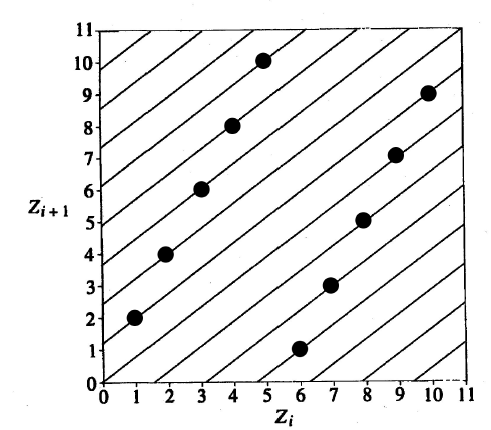
\includegraphics[width=0.5\textwidth]{img/14/korelacje.png}
        \label{fig:my_label}
    \end{figure}
\end{frame}
    \begin{frame}
	Kiedyś IBM wsławił się zdaniem: ``{\it gwarantuje tylko losowość każdej liczby indywidualnie }''
    \newline
    \newline
	b) {\it niższe bity są} ``{\it mniej losowe}'' niż {\it wyższe}:

    - nie wykorzystywać liczb losowych w {\it kawałkach},

	- np. do generowania liczb losowych $\in[1, 10 ]$

	używać:

	$J=1+INT(10.0*$RANF (iseed) $)$

	a nie:

	$J=1+MOD(INT(100000.0*RANF($iseed)$),\ 10)$
    \end{frame}

	%%%%%%%%%%%%%%%%
	\section{Zasady doboru stałych generatora liniowego kongruentnego}
	\begin{frame}{Zasady doboru stałych generatora liniowego kongruentnego}
Pojawiające sie w literaturze wnioski:\\ 
	\newline \newline
 	 $I_{0}$: \\
 	 - nie ma większego znaczenia\\
	
	$a$: \\
	- $a(mod 8)=5$ \\
	- $\frac{m}{100}<a<m-\sqrt{m}$ \\
	- brak powtarzającego się wzorca w zapisie w systemie dwójkowym
	\newline \newline
	$c$: \\
	- nieparzyste \\
 	- spełniające $ \frac{c}{m}\approx\frac{1}{2}-\frac{\sqrt{3}}{6}$
	\newline \newline
	$m$: \\
	$m=2^{t}$ , \quad t-liczba bitów przeznaczonych na 1 liczbę całkowitą


	\end{frame}

	%%%%%%%%%%%%%%%%
	\section{Zmniejszenie korelacji w sekwencji liczb losowych}
	\begin{frame}{Zmniejszenie korelacji w sekwencji liczb losowych}
	- procedura ''{\it losowego tasowania}'' (random shuffling procedure) {\it Bays-Durham 	$\Rightarrow Knuth$: ``The Art of Computer 	Programing'' vol. II.} 
	\newline 

	\textbf{RANF} - generator systemowy,

	\textbf{RANO} - generator ulepszony

	\textbf{A} - tablica pomocnicza o dlugosci wyznaczonej przez liczbę pierwszą)

\newline \newline
	Uogólnienie:

	- kilka generatorów

	- jeden z nich wybiera ``dostarczyciela'' liczb
	\end{frame}
    
	\begin{frame}{Zmniejszenie korelacji w sekwencji liczb losowych}
		\centering \includegraphics[width=.8\linewidth]{img/14/14_5_1_img.png}
	\end{frame}

	\begin{frame}{Zmniejszenie korelacji w sekwencji liczb losowych}
		\begin{enumerate}
			\setcounter{enumi}{-1}
			\item wypełniam tablicę $A$ i zmienną $x$ liczbami losowymi
			\item $x$ traktuje jak indeks $j$, który wskazuje na  element tablicy A 
			\item $A(j)$ wstawiam w miejsce $x$ oraz jednocześnie zwracam jako liczbę losową  ulepszonego generatora
			\item z generatora systemowego RANF losujemy  brakującą  liczbę w miejsce $A(j)$
		\end{enumerate}
	\end{frame}

	

	%%%%%%%%%%%%%%%%
	\section{Zmienne losowe o zadanym rozkładzie}
\subsection{Metoda  tranformacji}
\begin{frame}{Rozkład równomierny na (0,1) - dystrybuanta}
    Dystrybuanta jednoznacznie definiuje rozkład prawdopodobieństwa:
$$
F(x)=\int_{-\infty}^{x}{p(y)dy}
$$
Funkcja niemalejąca, określa  $P(X<x)$\\
Dla rozkładu równomiernego na (0,1), dla
$x\in (0,1)$ $p(x)=1$
$$
F(x)=\int_{-\infty}^{x}{p(y)dy}=x
$$
Czyli dla $x \in (0,1)$
$$P(X<x)=x$$
\end{frame}
\begin{frame}{Metoda odwróconej dystrybuanty}


Jak uzyskać rozkład o zadanej dystrubuancie $F(x)$ ?

Jeśli zdefiniujemy U - zmienną losową o rozkładzie równomiernym na (0,1) to zmienna losowa
$$
X=F^{-1}(U)
$$
ma rozkład o dystrybuancie $F(x)$\\

Dowód:
$$
P(X<x)= P(F^{-1}(U)<x
)=P(U<F(x))=F(x)
$$

\end{frame}
\begin{frame}{Przykład rozkład wykładniczy $e^{-x}$}
Funkcja gęstości prawdopodobieństwa:    
    $p(x)=e^{-x}$ $x \in [0,\infty)$\\
    
Dystrybuanta:
$$
F(x)=\int_{-\infty}^x{e^{-x'}dx'}=1-e^{-x}
$$
$$
y=1-e^{-x}
$$
$$
x=-ln(1-y)
$$
$$
F^{-1}(y)=-ln(1-y)
$$
Generujemy ciąg liczb losowych o rozkładzie równomiernym $U$ $u_1, u_2, u_3, .., u_n \in (0,1)$\\
Wtedy ciąg liczb:
$y_i=-ln(1-u_i)$
ma rozkład wykładniczy.\\
W ogólności odwracanie dystrybuanty sprawia często duże trudności numeryczne. 
\end{frame}
\begin{frame}{Rozkład normalny}
    $$p(x) = e^{-\frac{x^{2}}{2}} \quad, \qquad$$
    Szukanie odwrotności dystrybuanty(funkcja nieelementarna!):
    $$F(x)=\int_{-\infty}^{x}e^{\frac{-y^2}{2}}dy'=erf(x) $$
    jest kosztowne.
    
    Zwykle stosuje się metodę Boxa-Mullera 
\end{frame}

\begin{frame}{Metoda Box-Muller}

		Biorę dwa niezależne rozkłady normalne i liczę prawdopodobieńswo 
		łączne (iloczynu zdarzeń):
		
		$$
			p(x_1,x_2) = e^{-\frac{x_1^{2}}{2}}\cdot e^{-\frac{x_2^{2}}{2}}=
			e^{-\frac{x_1^{2}+x_2^{2}}{2}}
		$$	
	    $$
		x_1, x_2 \in (-\infty,\infty)
		$$
		Wprowadzamy zmienne sferyczne:
		$$
		r^2=x_1^{2}+x_2^{2}, r \in[0,\infty)
		$$
		$$
		x_1=r\sin(\phi), \phi \in [0, 2\pi]
		$$
		$$
		x_2=r\cos(\phi)
		$$
\end{frame}
\begin{frame}{Metoda Box-Muller}
    Przeliczamy element prawdopodobieństwa (prawdopodobieństwo, że x i y  znajdą się w małym obszarze dxdy) we współrzędnych sferycznych (\colorbox{red}{$r$} - moduł Jakobianu)
$$
p(x,y)dxdy=p(r,\phi)
\textrm{\colorbox{red}{$r$}}
d\phi dr
$$

$$
e^{-\frac{r^2}{2}} \textrm{\colorbox{red}{$r$}} d\phi dr
$$
Wprowadzam zmienną $z=\frac{r^2}{2}$
$$
dz=rdr
$$
$$
e^{-z}  d\phi dz
$$
\end{frame}
\begin{frame}{Metoda Box-Muller }
    Otrzymaliśmy rozkład wykładniczy $e^{-z}  d\phi dz$.\\
    Możemy zastosować odwrotną dystrubuantę:
    $$
F^{-1}(w)=-ln(1-w)
$$
oraz odwrotną funkcję do:
$\frac{r^2}{2}=z$ czyli $r=\sqrt{2z} $\\
    Dodatkowo gęstośc prawdopodobieństwa rozkładu $ e^{\frac{r^2}{2}}$  nie zależy od $\phi \in [0,2\pi]$, który losujemy zgodnie z rozkładem równomiernym na przedziale $(0,2\pi)$
   % $$
   %F(x)= \int_{-\infty}^{x}\int_{0}^{2\pi}e^{-z} % d\phi dz=2\pi \int_{-\infty}^{x}e^{-z} dz
   % $$
\end{frame}
\begin{frame}{Metoda Box-Muller}
	\begin{block}{Metoda Box-Muller  generacji zmiennych losowych o rozkładzie normalnym}
		\[
			p(r)dr = e^{-\frac{r^{2}}{2}}dr= e^{-\frac{x_1^{2}+x_2^2}{2}}dx_1dx_2=
			e^{-\frac{x_1^{2}}{2}}dx_1 e^{-\frac{x_2^{2}}{2}}dx_2
		\]
	\end{block}

	\begin{block}{transformacja:}
		$U_{1}, U_{2}$ - zm. losowe niezależne, rozkł. równomierny na $(0, 1)$
		\[
			x_{1} = r cos(\phi)=\sqrt{-2 \ln(1-U_1)} \cos(2\pi U_2)
		\]
		\[
			x_{2} = r sin(\phi)= \sqrt{-2 \ln(1-U_1)} \sin(2\pi U_2)
		\]
			$\Rightarrow$ $x_{1} x_{2}$ - każda oddzielnie ma rozkład normalny (2 niezależne!)
	\end{block}
\end{frame}
%%%%%%%%%%%%%%
%\begin{comment}
%\begin{frame}{Metoda Box-Muller (1958)}
%	\begin{block}{stąd:}
%		\[
%			x_{1} = \left[- \frac{1}{2} (y_{1}^{2} + y_{2}^{2})\right]
%		\]
%		\[
	%		x_{2} = \frac{1}{2\pi} \arctan\frac{y_{1}}{y_{2}}
%		\]
%	\end{block}
	
%	\begin{block}{co daje:}
	%	\[
		%	\frac{\partial(x_{1}, x_{2})}{\partial(y_{1}, y_{2})} = \begin{vmatrix}
		%		\frac{\partial x_{1}}{\partial y_{1}} & \frac{\partial x_{1}}{\partial y_{2}} \\
		%		\frac{\partial x_{2}}{\partial y_{1}} & \frac{\partial x_{2}}{\partial y_{2}}
		%	\end{vmatrix} =
		%	- \left[\frac{1}{\sqrt{2\pi}} e^{-\frac{y_{1}^{2}}{2}}\right] \left[\frac{1}{\sqrt{2\pi}} e^{-\frac{y_{2}^{2}}{2}}\right]
	%	\]
	%	$\Rightarrow$ $y_{1} y_{2}$ - każda oddzielnie ma rozkład normalny (2 niezależne!)
%	\end{block}
%\end{frame}
%\end{comment}
%%%%%%%%%%%%%%
\begin{frame}{Uproszczenie obliczeń}
	\begin{block}{Zamiast:}
		$U_{1}, U_{2}$ - rozkład równomierny w jednostkowym kwadracie
	\end{block}

	\begin{block}{bierzemy:}
		$V_{1}, V_{2}$ - współrz. punktu w jednostkowym kole:\\
		$V_{1}^{2} + V_{2}^{2} < 1$,\\
		zamiast $U_1$ bierzemy $R = V_{1}^{2} + V_{2}^{2}$ (też ma rozkład równomierny)\\
		zamiast $U_{2}$ - $\angle(V_{1}, V_{2})$ 
		\[
			\cos(2\pi U_{2}) = \frac{V_{1}}{\sqrt{R}}; \qquad \sin(2\pi U_{2}) = \frac{V_{2}}{\sqrt{R}}
		\]
		i tak unikamy stosowania funkcji trygonometrycznych
	\end{block}
\end{frame}
%%%%%%%%%%%%%%
\begin{frame}{Uproszczenie obliczeń}
	\begin{block}{}
		\[
			x_{1} = V_{1}\sqrt{\frac{-2 \ln(V_{1}^{2} + V_{2}^{2})}{V_{1}^{2} + V_{2}^{2}}},
		\]
		\[
			x_{2} = x_{1} \cdot \frac{V_{2}}{V_{1}}
		\]
		$x_{1}, x_{2}$ - niezależne, obie o $N(0,1)$
	\end{block}
\end{frame}
	%%%%%%%%%%%%%%%%
	\section{Kryptografia a liczby losowe}
\begin{frame}{Kryptografia a liczby losowe}
	Materiały dostępne w internecie:
	\begin{itemize}
		\item Quantifying Studies of (Pseudo) Random Number Generation for Cryptography\\
		\url{http://www.tcs.hut.fi/Publications/arock/these_roeck.pdf}
	\end{itemize}
	\end{frame}
	\begin{frame}{Mersenne Twister}
	\begin{itemize}
	 \item jeden z lepszych generatorów używanych obecnie 
	 \item  szybki 
	 \item dobre własności statystyczne  \item wada: stosunkowo duża liczba instrukcji z których się składa
	\end{itemize}
	
	\url{http://www.math.sci.hiroshima-u.ac.jp/m-mat/MT/ARTICLES/mt.pdf}
	
\end{frame}
	%%%%%%%%%%%%%%%%

\begin{frame}
		Źródło:

		N. E. Knuth, ``The Art of Computer Programing vol. II, Addison- Wesley, 1969.

		%G.E. Forsythe, M. A. Malcolm, C. R. Mcler, ``Computer Methods for Mathematical Computations 		Prentice Hall, 1977.

		 Wieczorkowski R., Zieliński R.: Komputerowe genaratory liczb losowych WNT 1997
\end{frame}

\end{document}
\grid
